%%%%%%%%%%%%%%%%%%%%%%%%%%%%%%%%%%%%%%%%%%%%%%%%%%%%%%%%%%%
%\section{Example cases}
%%%%%%%%%%%%%%%%%%%%%%%%%%%%%%%%%%%%%%%%%%%%%%%%%%%%%%%%%%%
%
%
%%%%%%%%%%%%%%%%%%%%%%%%%%%%%%%%%%%%%%%%%%%%%%%%%%%%%%%%%%%
\subsection{Collider bias: Berkson's paradox}
%%%%%%%%%%%%%%%%%%%%%%%%%%%%%%%%%%%%%%%%%%%%%%%%%%%%%%%%%%%
%
%
\begin{frame}[t, negative, label=sa]
	\subsectionpage
\end{frame}
%
%
\begin{frame}
	{Berkson's paradox\footnote{\citet{McElreath_2020}, chapter 6 (p. 161); \citet{Cinelli_et_al_2021} (p. 8)}}
	%
	\begin{columns}
		%
		\begin{column}{0.5\textwidth}
			%
			also known as,
			%
			\begin{itemize}
				%
				\item selection bias
				\item selection-distorsion effect
				\item \textcolor{blue}{``convenience" sample} bias
				%
			\end{itemize}
			
			research question, 
			%
			\begin{itemize}
				%
				\item \textcolor{blue}{Is there a true relationship between $N_{W}$ and $T_{W}$ in studies?}
				%
			\end{itemize}
			
			variables,
			%
			\begin{itemize}
				%
				\item $N_{W}$, ``news-worthiness" of a study 
				\item $T_{W}$, ``trust-worthiness" of a study 
				\item $S$, selected studies
				%
			\end{itemize}
			%
		\end{column}
		%
		\begin{column}{0.5\textwidth}  
			%
			\begin{equ}
				%
				M = \left\{ \begin{aligned} 
					T_{W} \leftarrow & \; f_{T}(U_{T}) \\
					N_{W} \leftarrow & \; f_{N}(U_{N}) \\
					S \leftarrow & \; f_{S}(T_{W}, N_{W}, U_{S}) \\
					U \sim & \; P(\pmb{U})
				\end{aligned} \right
				%
				\caption*{(a) structural model}
				%
			\end{equ}
			%
			\begin{figure}
				%
				\begin{tikzpicture}
					% nodes
					\node[formula] at (-2,0) {$U_{T}$};
					\node[formula] at (-1,-0.3) {$T_{W}$};
					\node[formula] at (1,1.5) {$U_{N}$};
					\node[formula] at (-0.15,1) {$N_{W}$};
					\node[formula] at (2,0) {$U_{S}$};
					\node[formula] at (1,-0.3) {$S$};
					
					% paths
					\draw [{Circle [open]}-{latex}{Circle}](-1.7,0)--(-0.9,0); % UT->T
					\draw [-{latex}](-0.9,0)--(0.9,0); %T->A
					\draw [{Circle [open]}-{latex}](0.9,1.3)--(0.1,0.8); % Un->N
					\draw [dashed, {latex}-{latex}](-0.95,0.05)--(0,0.75); % T->N
					\draw [{Circle [open]}-{latex}{Circle}](1.7,0)--(0.9,0); % Us->S
					\draw [{Circle}-{latex}](0,0.8)--(0.9,0.1); % N->S
					
					% extra
					\node at (-0.75,0.55) {$(?)$}; % symbol
				\end{tikzpicture}
				%
				\caption*{(b) causal diagram}
				%
			\end{figure}
			%
		\end{column}
		%
	\end{columns}
	%
\end{frame}
%
%
\begin{frame}
	{Simulation setting}
	%
	\begin{columns}
		%
		\begin{column}{0.5\textwidth}
			%
			\begin{figure}
				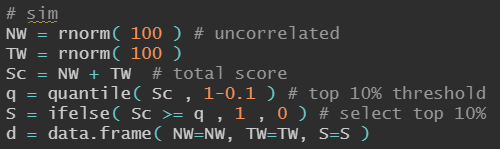
\includegraphics[scale=0.7]{collider1_code.png}
				\caption*{(c) R code}
			\end{figure}
			%
			\textcolor{blue}{Implications},
			%
			\begin{itemize}
				\item \dsep{$T_{W}$}{$N_{W}$} \\
				\item \ndsep{$T_{W}$}{$N_{W}$} \; | S
			\end{itemize}
			%
		\end{column}
		%
		\begin{column}{0.5\textwidth}  
			%
			\begin{equ}
				%
				M = \left\{ \begin{aligned} 
					T_{W} \leftarrow & \; f_{T}(U_{T}) \\
					N_{W} \leftarrow & \; f_{N}(U_{N}) \\
					S \leftarrow & \; f_{S}(T_{W}, N_{W}, U_{S}) \\
					U \sim & \; P(\pmb{U})
				\end{aligned} \right
				%
				\caption*{(a) structural model}
				%
			\end{equ}
			%
			\begin{figure}
				%
				\begin{tikzpicture}
					% nodes
					\node[formula] at (-2,0) {$U_{T}$};
					\node[formula] at (-1,-0.3) {$T_{W}$};
					\node[formula] at (1,1.5) {$U_{N}$};
					\node[formula] at (-0.15,1) {$N_{W}$};
					\node[formula] at (2,0) {$U_{S}$};
					\node[formula] at (1,-0.3) {$S$};
					
					% paths
					\draw [{Circle [open]}-{latex}{Circle}](-1.7,0)--(-0.9,0); % UT->T
					\draw [-{latex}](-0.9,0)--(0.9,0); %T->A
					\draw [{Circle [open]}-{latex}](0.9,1.3)--(0.1,0.8); % Un->N
					%\draw [dashed, {latex}-{latex}](-0.95,0.05)--(0,0.75); % T->N
					\draw [{Circle [open]}-{latex}{Circle}](1.7,0)--(0.9,0); % Us->S
					\draw [{Circle}-{latex}](0,0.8)--(0.9,0.1); % N->S
				\end{tikzpicture}
				%
				\caption*{(b) causal diagram}
				%
			\end{figure}
			%
		\end{column}
		%
	\end{columns}
	%
\end{frame}
%
%
\begin{lhframe}[rhgraphic={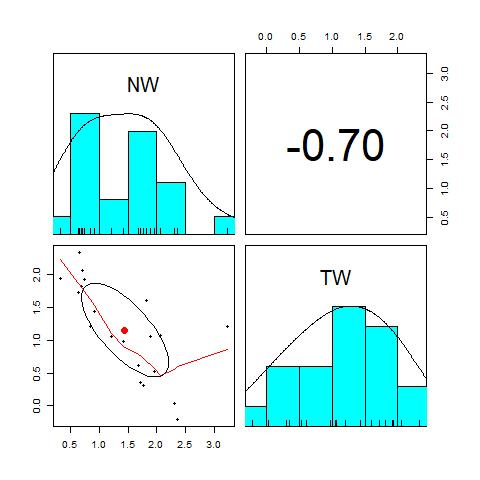
\includegraphics[scale=0.4]{collider1_panel2.jpg}}]
	{Descriptive analysis}
	
	based on \textcolor{blue}{descriptive analysis},
	%
	\begin{itemize}
		%
		\item what we observe is $Cor(N_{W}, T_{W} \; | \; S)$, \\
		{\small (data has been stratified on a score) }
		%
		\item $Cor(N_{W}, T_{W} \; | \; S)$ does NOT go in line with our ``rudimentary" understanding of the data\\
		{\small ($N_{W}$ and $T_{W}$ are related?)}
		%
		\item the issue is that we want to observe $Cor(N_{W}, T_{W})$ \\
		{\small (unconditional correlation)}
		%
	\end{itemize}
	%
\end{lhframe}
%
%
\begin{lhframe}[rhgraphic={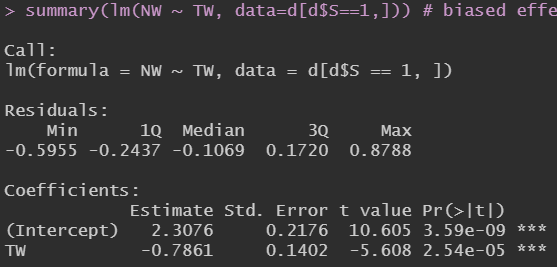
\includegraphics[scale=0.5]{collider1_reg1.png}}]
	{Regression does not solve anything!!}
	
	based on \textcolor{blue}{statistical analysis},
	%
	\begin{itemize}
		%
		\item $T_{W}$ continues to ``explain" $N_{W}$, \\
		{\small (is the only model accessible)}
		%
		\item But is it correct though?
		%
	\end{itemize}
	%
\end{lhframe}
%
%
\begin{lhframe}[rhgraphic={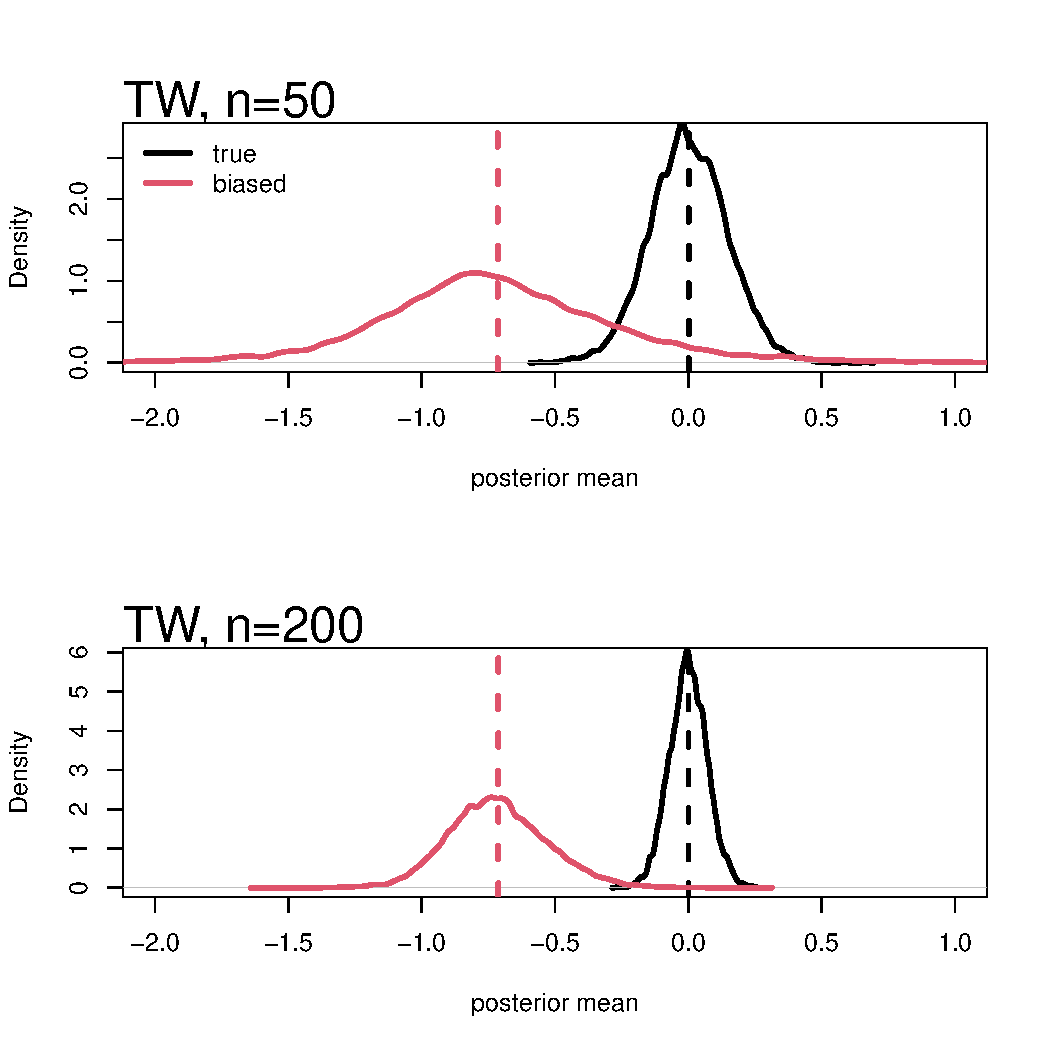
\includegraphics[scale=0.45]{collider1_samplesize.pdf}}]
	{Let me guess?, more data, more problems}
	
	imagine we can continue sampling,
	%
	\begin{itemize}
		%
		\item top: $10,000$ samples $n=20$
		\item bottom: $10,000$ samples $n=100$
		%
	\end{itemize}
	
	under the \textcolor{blue}{only available model}, \\
	the larger the sample size,
	%
	\begin{itemize}
		%
		\item the more \textcolor{blue}{certain} you are about your \textcolor{blue}{biased} estimates
		%
	\end{itemize}
	%
\end{lhframe}
%
%
\begin{lhframe}[rhgraphic={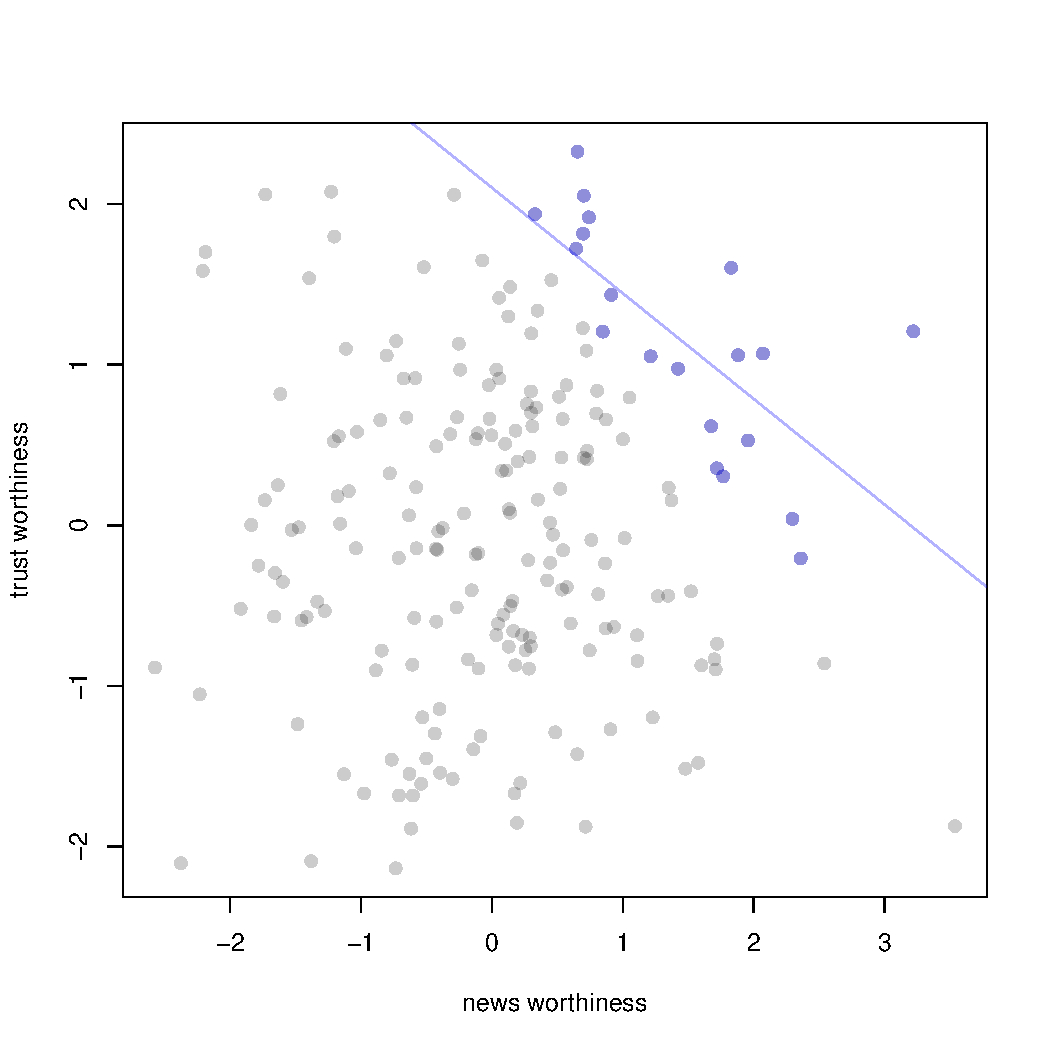
\includegraphics[scale=0.40]{collider1_triptych.pdf}}]
	{Ok, what is going on?}
	
	If we only observe data where $S=1$,
	%
	\begin{itemize}
		%
		\item it means that even if your study had a low $T_{W}$, you know it necessarily has a high $N_{W}$ to compensate and pass the threshold \\
		{\small (e.g. switch, electricity, and light)}
		%
	\end{itemize}
	%
\end{lhframe}
%
%
\begin{frame}
	{Similar case\footnote{\citet{Cinelli_et_al_2021} (p. 8)}}
	%
	\begin{columns}
		%
		\begin{column}{0.5\textwidth}
			
			research question, 
			%
			\begin{itemize}
				%
				\item \textcolor{blue}{Is there a true relationship between $NW$ and $TW$ in studies?}
				%
			\end{itemize}
			
			variables,
			%
			\begin{itemize}
				%
				\item $NW$, ``news-worthiness" of a study 
				\item $TW$, ``trust-worthiness" of a study 
				\item $U_{x}$, unobservable (e.g. no idea yet)
				\item $S$, selected studies
				%
			\end{itemize}
			%
		\end{column}
		%
		\begin{column}{0.5\textwidth}  
			%
			\begin{equ}
				%
				M = \left\{ \begin{aligned} 
					T_{W} \leftarrow & \; f_{T}(U_{T}) \\
					N_{W} \leftarrow & \; f_{N}(U_{N}) \\
					S \leftarrow & \; f_{S}(T_{W}, N_{W}, U_{S}) \\
					U \sim & \; P(\pmb{U})
				\end{aligned} \right
				%
				\caption*{(a) structural model}
				%
			\end{equ}
			%
			\begin{figure}
				%
				\begin{tikzpicture}
					% nodes
					\node[formula] at (-2,0) {$U_{T}$};
					\node[formula] at (-1,-0.3) {$T_{W}$};
					\node[formula] at (-1,1.5) {$U_{N}$};
					\node[formula] at (1,1.5) {$U_{X}$};
					\node[formula] at (-0,1.2) {$N_{W}$};
					\node[formula] at (2,0) {$U_{S}$};
					\node[formula] at (1,-0.3) {$S$};
					
					% paths
					\draw [{Circle [open]}-{latex}{Circle}](-1.7,0)--(-0.9,0); % Ut->T
					\draw [-{latex}](-0.9,0)--(0.9,0); %T->S
					\draw [{Circle [open]}-{latex}](1,1.3)--(0.1,0.8); % Ux->N
					\draw [{Circle [open]}-{latex}{Circle}](-1,1.25)--(0.1,0.75); % Un->N
					\draw [-{latex}](0.95,1.2)--(0.95,0.1); % Ux->S
					\draw [dashed, {latex}-{latex}](-0.95,0.05)--(0,0.75); % T->N
					\draw [{Circle [open]}-{latex}{Circle}](1.7,0)--(0.9,0); % Us->S
					
					
					% extra
					\node at (-0.75,0.55) {$(?)$}; % symbol
				\end{tikzpicture}
				%
				\caption*{(b) causal diagram}
				%
			\end{figure}
			%
		\end{column}
		%
	\end{columns}
	%
\end{frame}
%
%
\begin{frame}
	{Is there a way to fix it?}
	%
	\begin{columns}
		%
		\begin{column}{0.5\textwidth}
			%
			a simple ways,
			%
			\begin{itemize}
				%
				\item use a variable that closes the \textcolor{blue}{selection path}
				(2nd D-separation rule), \\
				i.e. stratify by a pipe to close the path \\
				$T_{W} \rightarrow Z \rightarrow S$ (see right) \\
				{\small or} \\
				$N_{W} \rightarrow Z \rightarrow S$ (not shown) \\
				$N_{W} \leftarrow U_{X} \rightarrow Z \rightarrow S$ (not shown)
				%
			\end{itemize}
			%
		\end{column}
		%
		\begin{column}{0.5\textwidth}  
			%
			\begin{figure}
				%
				\begin{tikzpicture}
					% nodes
					\node[formula] at (-2,0) {$U_{T}$};
					\node[formula] at (-1,-0.3) {$T_{W}$};
					\node[formula] at (1,1.5) {$U_{N}$};
					\node[formula] at (-0.15,1) {$N_{W}$};
					\node[formula] at (-0,-0.3) {$Z$};
					\node[formula] at (2,0) {$U_{S}$};
					\node[formula] at (1,-0.3) {$S$};
					
					% paths
					\draw [{Circle [open]}-{latex}](-1.7,0)--(-1.1,0); % Ut->T
					\draw [{Circle}-{latex}](-1.1,0)--(0,0); %T->Z
					\draw [{Circle[color=red]}-{latex}](0,0)--(0.9,0); %Z->S
					\draw [{Circle [open]}-{latex}](0.9,1.3)--(0.1,0.8); % Un->N
					\draw [dashed, {latex}-{latex}](-0.95,0.05)--(0,0.75); % T->N
					\draw [{Circle [open]}-{latex}{Circle}](1.7,0)--(0.9,0); % Us->S
					\draw [{Circle}-{latex}](0,0.8)--(0.9,0.1); % N->S
					
					% extra
					\node at (-0.75,0.55) {$(?)$}; % symbol
				\end{tikzpicture}
				%
				\caption*{(b1) causal diagram}
				%
			\end{figure}
			%
			\begin{figure}
				%
				\begin{tikzpicture}
					% nodes
					\node[formula] at (-2,0) {$U_{T}$};
					\node[formula] at (-1,-0.3) {$T_{W}$};
					\node[formula] at (-1,1.5) {$U_{N}$};
					\node[formula] at (1,1.5) {$U_{X}$};
					\node[formula] at (-0,1.2) {$N_{W}$};
					\node[formula] at (-0,-0.3) {$Z$};
					\node[formula] at (2,0) {$U_{S}$};
					\node[formula] at (1,-0.3) {$S$};
					
					% paths
					\draw [{Circle [open]}-{latex}](-1.7,0)--(-1.1,0); % Ut->T
					\draw [{Circle}-{latex}](-1.1,0)--(0,0); %T->Z
					\draw [{Circle[color=red]}-{latex}](0,0)--(0.9,0); %Z->S
					\draw [{Circle [open]}-{latex}](1,1.3)--(0.1,0.8); % Ux->N
					\draw [{Circle [open]}-{latex}{Circle}](-1,1.25)--(0.1,0.75); % Un->N
					\draw [-{latex}](0.95,1.2)--(0.95,0.1); % Ux->S
					\draw [dashed, {latex}-{latex}](-0.95,0.05)--(0,0.75); % T->N
					\draw [{Circle [open]}-{latex}{Circle}](1.7,0)--(0.9,0); % Us->S
					
					
					% extra
					\node at (-0.75,0.55) {$(?)$}; % symbol
				\end{tikzpicture}
				%
				\caption*{(b2) causal diagram}
				%
			\end{figure}
			%
		\end{column}
		%
	\end{columns}
	%
\end{frame}
%
%
\begin{lhframe}[rhgraphic={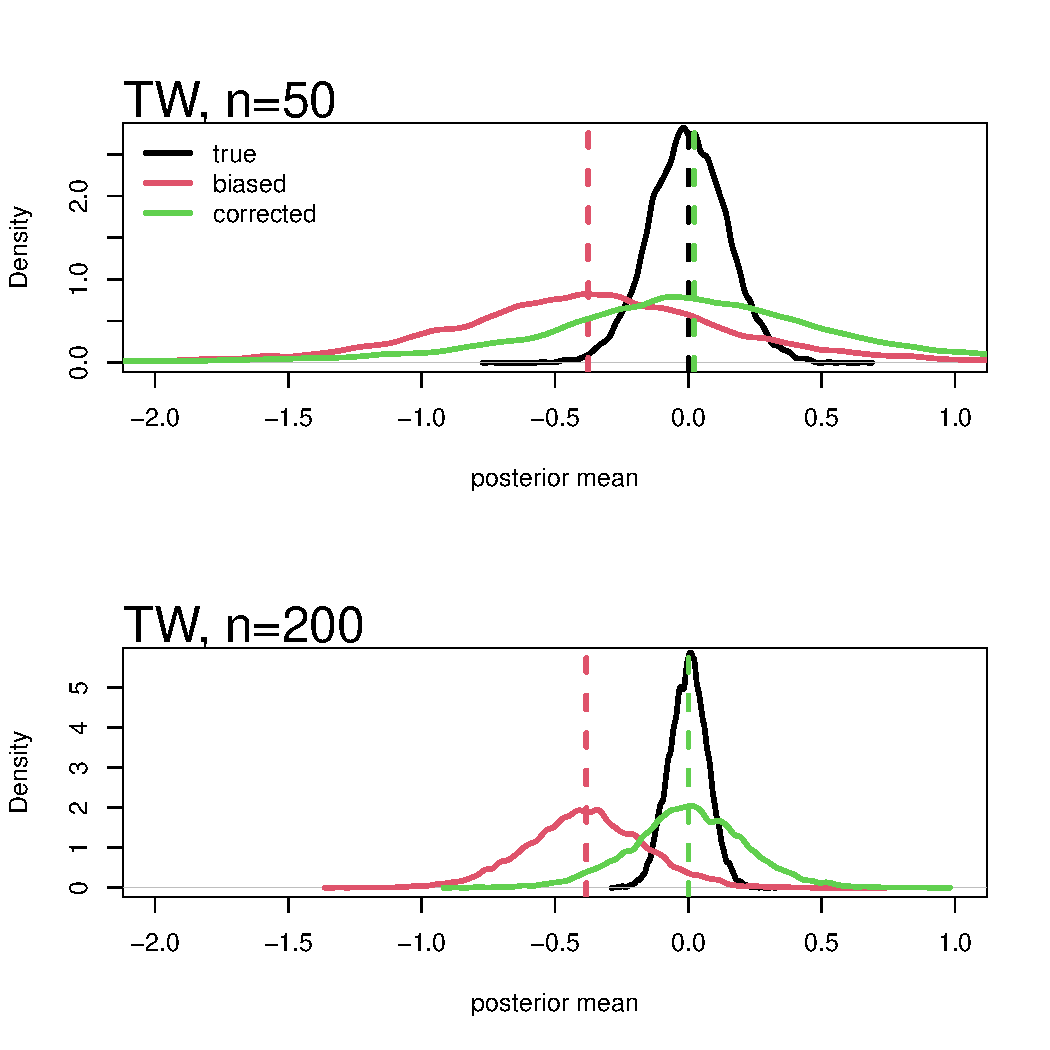
\includegraphics[scale=0.5]{collider1_samplesize2.pdf}}]
	{Does it work though?}
	
	based on the previous \textcolor{blue}{DAGs}, \\
	the \textcolor{blue}{statistical analysis} reveals,
	%
	\begin{itemize}
		%
		\item stratifying by $Z$ ``corrects" the estimates, \\
		{\small (but we still lose some precision) }
		%
	\end{itemize}
	%
\end{lhframe}
%
%
\begin{frame}
	{Other ways to solve it?\footnote{most also apply for previous examples, but are beyond the scope of this document (for now)}}
	
	many other (much more complex) ways,
	%
	\begin{itemize}
		%
		\item sensitivity analysis \\
		{\small (example \hyperlink{sa}{here})}
		%
		\item post-stratification? \\
		{\small (example \hyperlink{sa}{here})}
		%
		\item matching?
		%
		\item inverse-probability weighting?
		%
		\item g-formula?
		%
		\item g-estimations?
		%
	\end{itemize}
	%
\end{frame}
%
%
%%%%%%%%%%%%%%%%%%%%%%%%%%%%%%%%%%%%%%%%%%%%%%%%%%%%%%%%%%%
\subsection{Collider bias: M-bias}
%%%%%%%%%%%%%%%%%%%%%%%%%%%%%%%%%%%%%%%%%%%%%%%%%%%%%%%%%%%
%
%
\begin{frame}[t, negative]
	\subsectionpage
\end{frame}
%
%
\begin{frame}
	{M-bias\footnote{\citet{McElreath_2022}, lecture 6; \citet{Cinelli_et_al_2021} (p. 4)}}
	%
	\begin{columns}
		%
		\begin{column}{0.5\textwidth}
			%
			case of,
			%
			\begin{itemize}
				%
				\item bias on pre-treatment variable
				%
			\end{itemize}
			
			research question, 
			%
			\begin{itemize}
				%
				\item \textcolor{blue}{Should we include $Z$ in our model?}
				%
			\end{itemize}
			
			variables,
			%
			\begin{itemize}
				%
				\item $Z$, ``health" quality of friends \\
				{\small (defined as a continuum)}
				\item $X$, health of individual $1$
				\item $U_{1}$, hobbies of individual $1$
				\item $Y$, health of individual $2$
				\item $U_{2}$, hobbies of individual $2$ 
				%
			\end{itemize}
			%
		\end{column}
		%
		\begin{column}{0.5\textwidth}  
			%
			\begin{equ}
				%
				M = \left\{ \begin{aligned} 
					X \leftarrow & \; f_{X}(U_{1},U_{X}) \\
					Z \leftarrow & \; f_{Z}(U_{1},U_{2},U_{Z}) \\
					Y \leftarrow & \; f_{Y}(X, U_{2}, U_{Y}) \\
					U \sim & \; P(\pmb{U})
				\end{aligned} \right
				%
				\caption*{(a) structural model}
				%
			\end{equ}
			%
			\begin{figure}
				%
				\begin{tikzpicture}
					% nodes
					\node[formula] at (-1,1) {$U_{1}$};
					\node[formula] at (-2,0) {$U_{X}$};
					\node[formula] at (-1,-0.3) {$X$};
					\node[formula] at (1,1.7) {$U_{Z}$};
					\node[formula] at (-0.1,1.05) {$Z$};
					\node[formula] at (1,1) {$U_{2}$};
					\node[formula] at (2,0) {$U_{Y}$};
					\node[formula] at (1,-0.3) {$Y$};
					
					% paths
					\draw [{Circle[open]}-{latex}](-0.95,0.8)--(-0.95,0.05); % U1->X
					\draw [-{latex}{Circle}](-0.9,0.75)--(0,0.75); % U1->Z
					\draw [{Circle[open]}-{latex}{Circle}](-1.7,0)--(-0.9,0); % Ux->X
					\draw [-{latex}](-0.9,0)--(0.9,0); % X->Y
					\draw [{Circle [open]}-{latex}{Circle}](1.7,0)--(0.9,0); % Uy->y
					\draw [{Circle [open]}-{latex}](0.9,1.5)--(0,0.8); % Uz->Z
					\draw [-{latex}](0.90,0.75)--(0,0.75); % U2->Z
					\draw [{Circle[open]}-{latex}](0.95,0.8)--(0.95,0.05); % U2->Y
					
					% extra
					\node at (0,-0.25) {$(?)$}; % symbol
				\end{tikzpicture}
				%
				\caption*{(b) causal diagram}
				%
			\end{figure}
			%
		\end{column}
		%
	\end{columns}
	%
\end{frame}
%
%
\begin{frame}
	{Simulation setting}
	%
	\begin{columns}
		%
		\begin{column}{0.5\textwidth}
			%
			\begin{figure}
				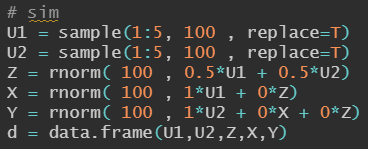
\includegraphics[scale=0.8]{collider2_code.png}
				\caption*{(c) R code}
			\end{figure}
			%
			\textcolor{blue}{Implications},
			%
			\begin{itemize}
				\item \dsep{X}{Y} \\
				\item \ndsep{X}{Y} \; | Z 
			\end{itemize}
			%
		\end{column}
		%
		\begin{column}{0.5\textwidth}  
			%
			\begin{equ}
				%
				M = \left\{ \begin{aligned} 
					X \leftarrow & \; f_{X}(U_{1},U_{X}) \\
					Z \leftarrow & \; f_{Z}(U_{1},U_{2},U_{Z}) \\
					Y \leftarrow & \; f_{Y}(X, U_{2}, U_{Y}) \\
					U \sim & \; P(\pmb{U})
				\end{aligned} \right
				%
				\caption*{(a) structural model}
				%
			\end{equ}
			%
			\begin{figure}
				%
				\begin{tikzpicture}
					% nodes
					\node[formula] at (-1,1) {$U_{1}$};
					\node[formula] at (-2,0) {$U_{X}$};
					\node[formula] at (-1,-0.3) {$X$};
					\node[formula] at (1,1.7) {$U_{Z}$};
					\node[formula] at (-0.1,1.05) {$Z$};
					\node[formula] at (1,1) {$U_{2}$};
					\node[formula] at (2,0) {$U_{Y}$};
					\node[formula] at (1,-0.3) {$Y$};
					
					% paths
					\draw [{Circle[open]}-{latex}](-0.95,0.8)--(-0.95,0.05); % U1->X
					\draw [-{latex}{Circle}](-0.9,0.75)--(0,0.75); % U1->Z
					\draw [{Circle[open]}-{latex}{Circle}](-1.7,0)--(-0.9,0); % Ux->X
					%\draw [-{latex}](-0.9,0)--(0.9,0); % X->Y
					\draw [{Circle [open]}-{latex}{Circle}](1.7,0)--(0.9,0); % Uy->y
					\draw [{Circle [open]}-{latex}](0.9,1.5)--(0,0.8); % Uz->Z
					\draw [-{latex}](0.90,0.75)--(0,0.75); % U2->Z
					\draw [{Circle[open]}-{latex}](0.95,0.8)--(0.95,0.05); % U2->Y
				\end{tikzpicture}
				%
				\caption*{(b) causal diagram}
				%
			\end{figure}
			%
		\end{column}
		%
	\end{columns}
	%
\end{frame}
%
%
\begin{lhframe}[rhgraphic={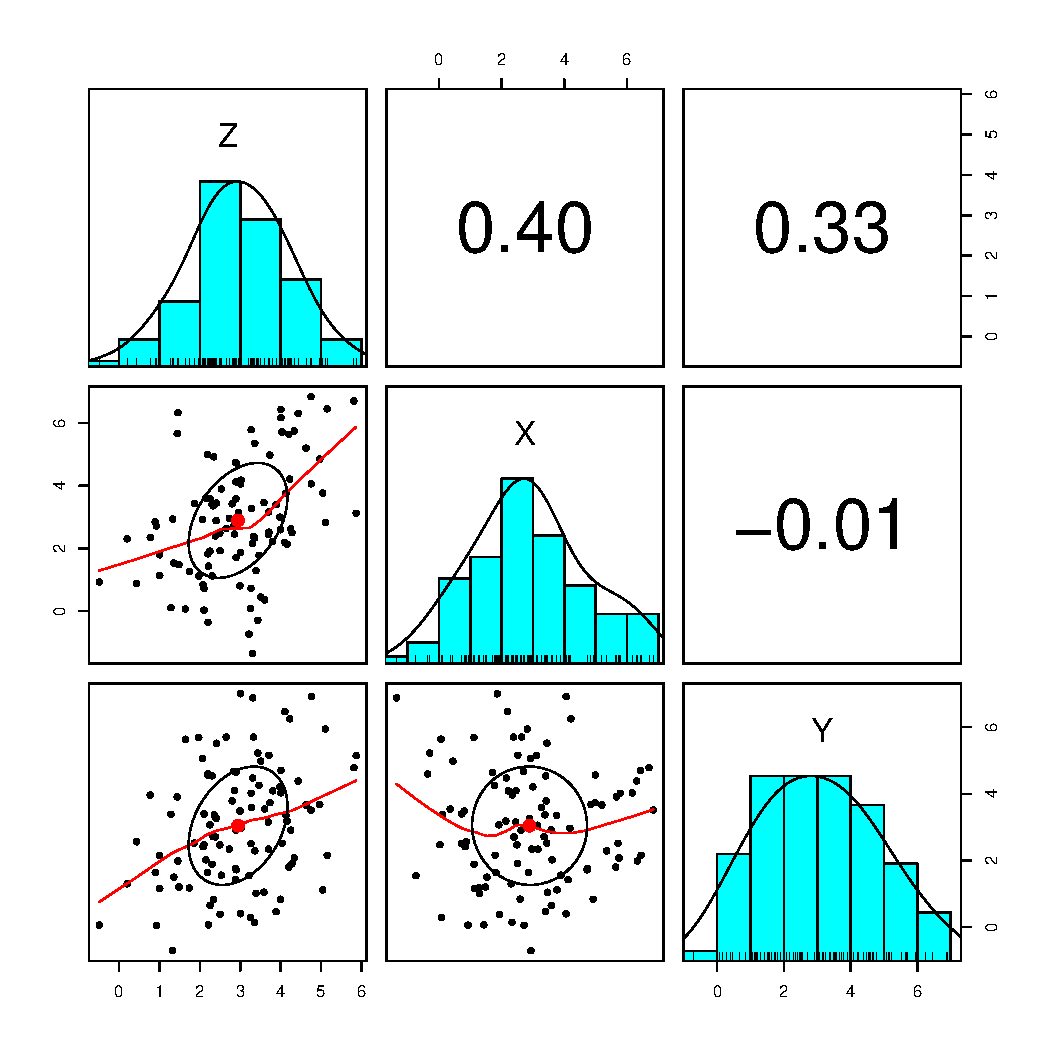
\includegraphics[scale=0.40]{collider2_panel.pdf}}]
	{Descriptive analysis}
	
	based on \textcolor{blue}{descriptive analysis},
	%
	\begin{itemize}
		%
		\item $Cor(X, Y) \approx 0$, quite low
		%
		\item larger $Cor(Z,Y)$, while $Cor(Z,X)$ is not high enough to discard it as a cause of multicollinearity,
		%
		\item we \textcolor{blue}{might include} $Z$ rather than $X$ \\
		{\small (but the effect of $X$ is our interest!!)}
		%
		\item then we include $Z$ and $X$
		%
	\end{itemize}
	%
\end{lhframe}
%
%
\begin{lhframe}[rhgraphic={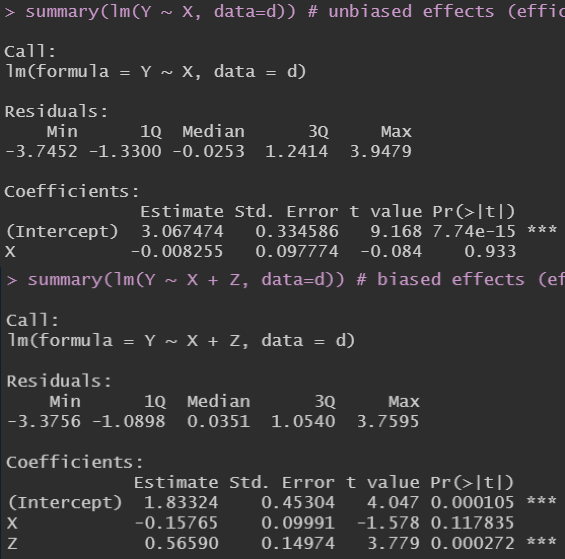
\includegraphics[scale=0.3]{collider2_reg.png}}]
	{Again regression!!}
	
	based on \textcolor{blue}{statistical analysis},
	%
	\begin{itemize}
		%
		\item $X$ does not have an effect of $Y$, \\
		{\small (in the first nor the second model)}
		%
		\item but $X$ has an (non-negligible) effect when $Z$ is in the model \\
		{\small (but we do not reject the null)}
		%
		\item The increase of the $X$ effect might lead you to think that with more data, we can reject the null \\
		{\small (and you would be right!!)} \\
		%
		\item But is it correct to include $Z$?
		%
	\end{itemize}
	%
\end{lhframe}
%
%
\begin{lhframe}[rhgraphic={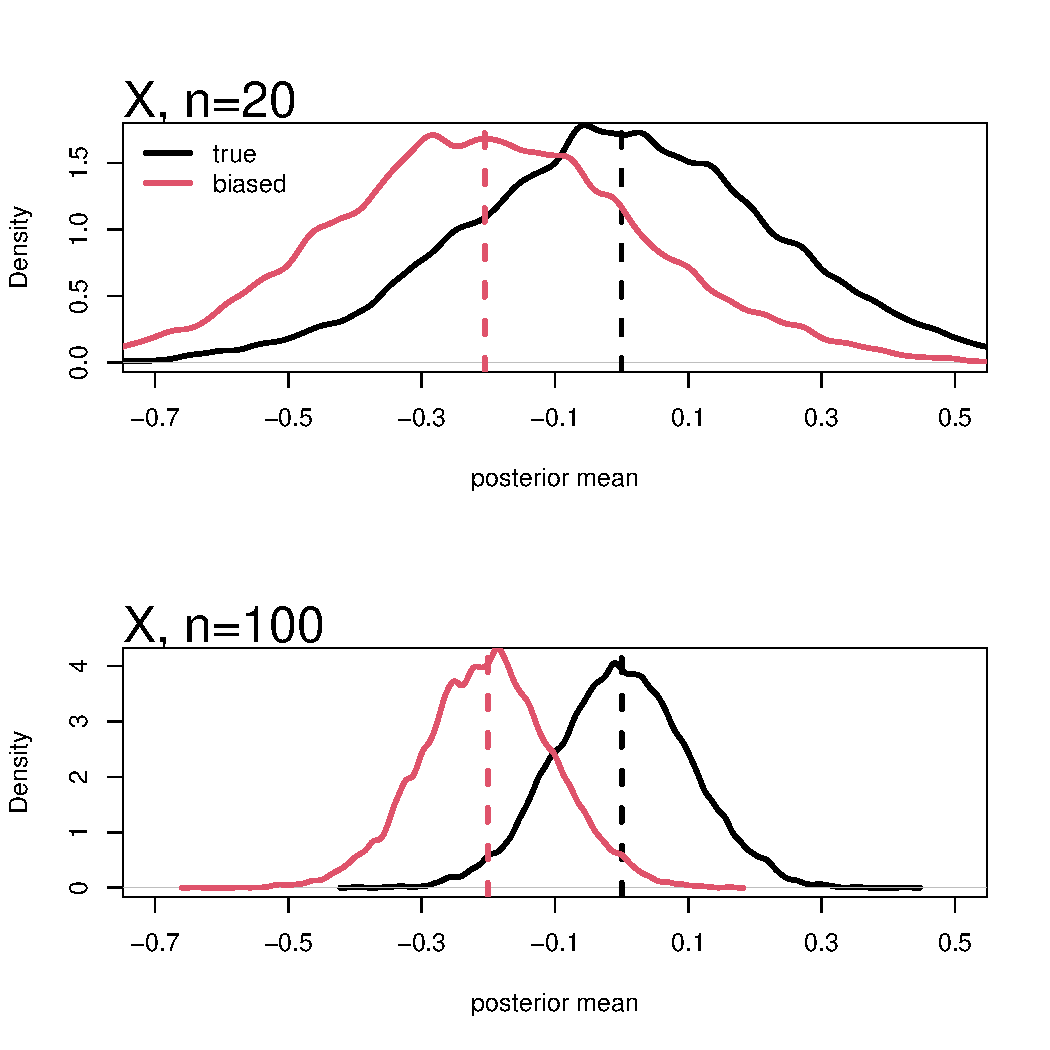
\includegraphics[scale=0.45]{collider2_samplesize.pdf}}]
	{Ok, I get it!!, more data, more wrong!!}
	
	imagine we can continue sampling,
	%
	\begin{itemize}
		%
		\item top: $10,000$ samples $n=20$
		\item bottom: $10,000$ samples $n=100$
		%
	\end{itemize}
	
	under the \textcolor{blue}{``incorrect" model}, \\
	the larger the sample size,
	%
	\begin{itemize}
		%
		\item the more \textcolor{blue}{certain} you are about your \textcolor{blue}{biased} estimates \\
		{\small (with enough you could reject the null)}
		%
	\end{itemize}
	%
\end{lhframe}
%
%
\begin{frame}
	{The dream team strikes back!!}
	%
	\begin{columns}
		%
		\begin{column}{0.5\textwidth}
			%
			based on \textcolor{blue}{DAG} and \textcolor{blue}{statistical model},
			%
			\begin{itemize}
				%
				\item the 3rd D-separation states that a collider that has been conditioned on \textcolor{blue}{does not block a path}, \\
				in this case: $X \rightarrow U_{1} \rightarrow Z \rightarrow U_{2} \rightarrow Y$ \\
				i.e. \ndsep{X}{Y} \; | Z \\
				%
				\item therefore if we want to find the direct effect of $X \rightarrow Y$, we \textcolor{blue}{should not} stratify by $Z$
				%
			\end{itemize}
			%
		\end{column}
		%
		\begin{column}{0.5\textwidth}  
			%
			\begin{equ}
				%
				M = \left\{ \begin{aligned} 
					X \leftarrow & \; f_{X}(U_{1},U_{X}) \\
					Z \leftarrow & \; f_{Z}(U_{1},U_{2},U_{Z}) \\
					Y \leftarrow & \; f_{Y}(X, U_{2}, U_{Y}) \\
					U \sim & \; P(\pmb{U})
				\end{aligned} \right
				%
				\caption*{(a) structural model}
				%
			\end{equ}
			%
			\begin{figure}
				%
				\begin{tikzpicture}
					% nodes
					\node[formula] at (-1,1) {$U_{1}$};
					\node[formula] at (-2,0) {$U_{X}$};
					\node[formula] at (-1,-0.3) {$X$};
					\node[formula] at (1,1.7) {$U_{Z}$};
					\node[formula] at (-0.1,1.05) {$Z$};
					\node[formula] at (1,1) {$U_{2}$};
					\node[formula] at (2,0) {$U_{Y}$};
					\node[formula] at (1,-0.3) {$Y$};
					
					% paths
					\draw [{Circle[open]}-{latex}](-0.95,0.8)--(-0.95,0.05); % U1->X
					\draw [-{latex}{Circle}](-0.9,0.75)--(0,0.75); % U1->Z
					\draw [{Circle[open]}-{latex}{Circle}](-1.7,0)--(-0.9,0); % Ux->X
					\draw [-{latex}](-0.9,0)--(0.9,0); % X->Y
					\draw [{Circle [open]}-{latex}{Circle}](1.7,0)--(0.9,0); % Uy->y
					\draw [{Circle [open]}-{latex}](0.9,1.5)--(0,0.8); % Uz->Z
					\draw [-{latex}](0.90,0.75)--(0,0.75); % U2->Z
					\draw [{Circle[open]}-{latex}](0.95,0.8)--(0.95,0.05); % U2->Y
					
					% extra
					\node at (0,-0.25) {$(?)$}; % symbol
				\end{tikzpicture}
				%
				\caption*{(b) causal diagram}
				%
			\end{figure}
			%
		\end{column}
		%
	\end{columns}
	%
\end{frame}
%
%
\begin{lhframe}[rhgraphic={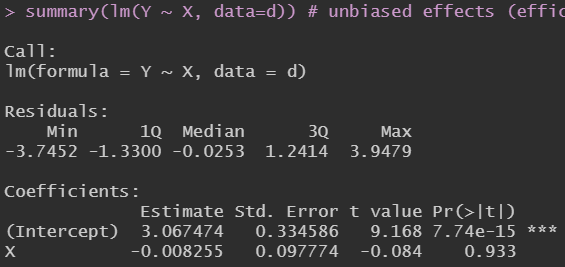
\includegraphics[scale=0.5]{collider2_reg1.png}}]
	{The dream team strikes back!!}
	
	based on \textcolor{blue}{DAG} and \textcolor{blue}{statistical analysis},
	%
	\begin{itemize}
		%
		\item the model that answers our research question is the first one, \\
		{\small \textcolor{blue}{(assuming our DAG is true)} }
		%
	\end{itemize}
	%
\end{lhframe}
%
%